\documentclass[red,unicode]{beamer}
\usepackage[utf8]{inputenc}
\usepackage[russian]{babel}
\usepackage{cmap,pscyr}
\usepackage{upgreek}
\usepackage{graphicx}
\usepackage{tikz,tabularx,booktabs,colortbl}
\usepackage{listings}
\lstdefinestyle{mystyle}{language=Python,
numbers=left,
numberstyle=\tiny\color{linenum},
numbersep=5.5pt,
keywordstyle=\bf\color{keywords}}
\lstdefinelanguage{morepython}
{morekeywords={map,sorted}}
\usetikzlibrary{shapes,snakes,trees,calc,fit,shadows,arrows,positioning,matrix}
\pgfdeclarelayer{background}
\pgfdeclarelayer{foreground}
\pgfsetlayers{background,main,foreground}


\definecolor{linenum}{rgb}{0.5,0.2,0.7}
\definecolor{keywords}{rgb}{0.28,0.1,0.3}
\definecolor{firstlevel}{rgb}{0.4,0,0}
\definecolor{secondlevel}{rgb}{0.7,0,0}
\definecolor{thirdlevel}{rgb}{1,0,0}
\definecolor{main}{rgb}{0.6,0.1,0.45}

\usetheme{Warsaw}

\setbeamercolor{block body}{bg=main!5} 
\setbeamercolor*{palette primary}{use=structure,fg=white,bg=main}
\newcommand{\bfc}{\bf\color{main!80!black}}
\usepackage[margin=15pt,font={small,sf,it},labelfont=bf]{caption} 
\usebackgroundtemplate{
\includegraphics[width=\paperwidth]{drawing.png}}
\useoutertheme[subsection=false]{smoothbars}
\title[Машинное обучение]{Классификация. Метод ближайших соседей (kNN). Машины опорных векторов (SVM)}
\author{Сергей Лисицын}
\institute{lisitsyn.s.o@gmail.com}
\date{22 марта 2011 г.}
\setbeamertemplate{footline}[page number]{}
\setbeamertemplate{navigation symbols}{}

\setbeamersize{text margin left=1.5em,text margin right=1.5em}
\setbeamertemplate{itemize item}{$\bullet$}
\setbeamertemplate{itemize subitem}{$\bullet$}
\setbeamertemplate{enumerate items}[default]

\setbeamercolor{enumerate item}{bf=black,fg=main}  
\setbeamercolor{itemize item}{fg=main}  
\setbeamercolor{enumerate subitem}{bf=white,fg=main}  
\setbeamercolor{itemize subitem}{fg=main}  

\begin{document}
\section{}
\abovedisplayskip=.6\abovedisplayskip
\belowdisplayskip=.6\belowdisplayskip

\begin{frame}

\titlepage
\end{frame}


\begin{frame}{Задача классификации}{classification}
\begin{itemize}
	\item $\sim$ задача распознавания образов
	\item Имеется некоторое пространство объектов
	\item Объекты разделены каким-либо образом на классы -- непересекающиеся множества схожих объектов
	\item Известны классы некоторых из объектов (прецеденты)
	\item Решение задачи -- алгоритм, позволяющий определить класс для любого элемента пространства объектов на основе имеющихся прецедентов
	\item В некоторых случаях необходимо определение вероятностей классов
\end{itemize}
\end{frame}

\section{Общие понятия}
\subsection{}
\begin{frame}{Общая задача классификации}
Пусть имеется некоторое множество объектов $\mathcal{X}$, конечное множество классов $\mathcal{C}$ и определено отображение
$$
f: \mathcal{X} \to \mathcal{C},
$$
причём известно, что некоторым элементам $X \subset \mathcal{X}$ соответствуют некоторые классы из множества $\mathcal{C}$. Множество
$$
\left \{ X, f(X) \right\} = \left\{ ( x_i, f (x_i) ) \right\}_{i=1}^{N}
$$ 
называется обучающей выборкой.\\[0.5cm]
{\bfc Задача классификации} состоит в нахождении функции $\hat f$, аппроксимирующей $f$ на всех элементах $\mathcal{X}$, которая позволит любой объект из $\mathcal{X}$ отнести к некоторому классу из $\mathcal{C}$.
\end{frame}

\begin{frame}{Для чего это нужно?}{}
\begin{itemize}
	\item Распознавание изображений
	\item Поддержка решений в банковской сфере
	\item Дифференциальная диагностика
	\item Классификация документов
	\item Анализ геостатистической информации
	\item Другие задачи, требующие <<узнавания объектов>>
\end{itemize}
\end{frame}


\begin{frame}{Качество классификации}
\begin{itemize}
	\item На каждом объекте $x$ из обучающей выборки $(X,f(X))$ можно вычислить функцию потерь построенного алгоритма $\hat f$
$$
L_{\hat f} (x) = [\hat f(x) \ne f(x)]
$$
	\item Средняя сумма ошибок на всей обучающей выборке $x_1, \dots, x_N$ -- эмпирический риск -- даёт понятие о качестве построенного алгоритма
$$
\hat R (\hat f) = \frac{1}{N} \sum_{i=1}^{N} L_{\hat f} (x_i)
$$
	\item Вполне ясно, что лучше этот риск минимизировать
	\item В вычислительной теории обучения эта мысль формализована в принцип минимизации эмпирического риска
\end{itemize}
\end{frame}

\begin{frame}{Принцип минимизации эмпирического риска}{Empirical Risk Minimization (ERM) principle}
\begin{itemize}
	\item Функционал эмпирического риска $\hat R(\hat f)$ должен минимизироваться, чтобы обеспечить максимально возможно высокое качество на любых данных
	\item Минимизация риска встречается даже в статистике
	\begin{itemize}
		\item $\hat R(\hat f) = \frac{1}{N} \sum_{i=1}^{N} (y_i - \hat f(x_i))^2 \to \min$   -- метод наименьших квадратов
		\item $\hat R(\hat p) = -\frac{1}{N} \sum_{i=1}^{N} \ln \hat p(x_i) \to \min$ -- метод максимального правдоподобия Фишера

	\end{itemize}
%	\item В работах Вапника показаны границы для среднего риска при заданной 
	\item Однако, безусловный минимум риска почти никогда не даст правильного алгоритма классификации, он слишком приспособлен к обучающим данным

\end{itemize}
\end{frame}


\begin{frame}{Обобщающая способность алгоритма классификации}{Generalization ability}
\begin{itemize}
	\item Хороший алгоритм классификации не только допускает мало ошибок на обучающей выборке, но и мало ошибается на любых других данных
	\item Обобщающей способностью алгоритма называется его способность допускать мало ошибок на тестовых данных после обучения 
	\item Теоретические оценки обобщающей способности чрезвычайно завышены и пока не могут дать ответа о применимости конкретных алгоритмов обучения к конкретным данным
	\item На практике оценить обобщающую способность можно с помощью скользящего контроля по обучающей выборке
\end{itemize}
\end{frame}


\begin{frame}{Скользящий контроль}{Cross validation (CV)}
\begin{itemize}
	\item Процедура скользящего контроля позволяет оценить насколько хорошо алгоритм обучения обобщает данные. Суммарная ошибка

$$
CV (\mu, \mathcal{X})= \sum_{\mathcal{X}_1,\mathcal{X}_2: \mathcal{X}_1 \cup \mathcal{X}_2 = \mathcal{X}} Q\Bigl(\underbrace{~~~~\mu(\mathcal{X}_1)~~~~}_{\substack{ \text{алгоритм,} \\ \text{построенный на} \\ \text{основе выборки $\mathcal{X}_1$}}},\mathcal{X}_2\Bigr)
$$

	\item Контроль по $q$ блокам (q-fold CV) разбивает обучающую выборку на $q$ непересекающихся подмножеств 


	\item Минимум функции ошибки на скользящем контроле важен для настройки параметров алгоритмов и вообще оценки качества
\end{itemize}
\end{frame}

\begin{frame}{Переобучение и недообучение}{Overfitting, underfitting}
\begin{itemize}
	\item Алгоритм вполне может не допускать ошибок на обучающей выборке вообще, но при этом суммарная ошибка скользящего контроля и его результаты на других данных катастрофически плохи. Такое явление называется переобучением (overfitting)

	\item С другой стороны, алгоритм может одинаково плохо работать как на обучающей выборке, так и на реальных данных -- в этом случае алгоритм недообучается (underfitting)

	\item Для хорошего качества алгоритма необходимо избегать этих крайностей
\end{itemize}
\end{frame}

\begin{frame}{Принципы MLE и MAP}{maximum likelihood estimation (MLE), maximum a posteriori (MAP)}
\begin{itemize}
\item Метод максимального правдоподобия (MLE): условная вероятность данных при гипотезе максимизируется
$$
\hat h = \arg\max_h P(\mathcal{D}|h)
$$
\item Принцип максимальной апостериорной вероятности (MAP): условная вероятность гипотезы при данных максимизируется
$$
\hat h = \arg\max_h P(h|\mathcal{D})
$$
\end{itemize}
\end{frame}

\begin{frame}{Принцип максимальной апостериорной вероятности для классификации}{MAP classification}
\begin{itemize}
	\item В случае классификации гипотеза -- принадлежность классифицируемого объекта некоторому классу

	\item Оптимальным классификатором с точки зрения MAP и ERM является
$$
\hat f(x) = \arg\max_{c \in \mathcal{C}} P(c | x)
$$
	\item Саму функцию вероятности $P(c|x)$ найти по обучающей выборке не представляется возможным, приходится находить её каким-то иным образом
\end{itemize}
\end{frame}

\section{Метод ближайших соседей}
\subsection{}

\begin{frame}{Классификация с помощью метода ближайших соседей}
\begin{itemize}
	\item Вся идея алгоритма состоит в аппроксимации апостериорной вероятности класса $P(c|x)$ через объекты обучающей выборки и расстояния до них
	\item Рассуждение по прецедентам (case-based reasoning) хорошо объясняет ответ, полученный алгоритмом
	\item Относится к классу алгоритмов ленивого обучения (lazy learning): обучение алгоритма сводится к <<запоминанию>> обучающей выборки
	\item Необходима метрика между всеми объектами, то есть пространство должно быть метрическим и не содержать категориальных и бинарных признаков
\end{itemize}
\end{frame}

%\begin{frame}{Метрические пространства}{}
%{\bfcМетрическое пространство} --- множество $\mathcal{X}$ с определённой на %нём функцией -- метрикой, являющейся отображением
%$$
%\rho: \mathcal{X} \times \mathcal{X} \to \mathbb{R}
%$$
%Метрика должна удовлетворять следующим четырём аксиомам
%\begin{enumerate}
%\item $\rho(x,y) \geqslant 0$ -- метрика всегда неотрицательна
%\item $\rho(x,y) = 0$ тогда и только тогда, когда $x=y$
%\item $\rho(x,y) = \rho(y,x)$ -- метрика симметрична
%\item $\rho(x,y) \leqslant \rho(x,z) + \rho(z,y)$ -- неравенство %треугольника\footnote{\scriptsizeиногда пренебрегается на практике}
%\end{enumerate}
%\end{frame}

\begin{frame}{Метрические пространства}
\begin{itemize}
	\item Метрическое пространство -- множество, с определённой на нём функцией $\rho(x,y)$ -- метрикой
	\item Метрика должна быть неотрицательной, симметричной и для неё должно выполняться неравенство треугольника
	\item Примеры метрик:
\begin{enumerate}
	\item Метрика Минковского (при $p=1$ -- метрика Манхэттена (city-block), при $p=2$ -- евклидова)
		$$
		\rho (x,y) = \left(\sum_i \left|x_i - y_i\right|^p \right)^{\frac{1}{p}}
		$$
	\item Расстояние Махаланобиса
		$$
		\rho (x,y) = \sqrt{(x-y)^{\mathsf{T}} S^{-1} (x-y)},
		$$
\end{enumerate}
\end{itemize}
\end{frame}


%\begin{frame}{Классификация с помощью метрики}
%\begin{itemize}
%	\item Проклятие размерности (curse of dimensionality): при размерности %пространства $N \to \infty$ метрика перестаёт быть эффективной функцией %схожести объектов
%	\item Зависимость от выбора метрики: неадекватный выбор метрики %чрезвычайно ухудшает качество классификации. Автоматический выбор метрики %ограничивается необходимостью перебора без каких-либо эвристик и небольшим %количеством известных метрик
%	\item Несмотря на эвристичность, схожа с задачей восстановления плотности распределения по данной выборке (в случае парзеновских окон вообще в неё вырождается)
%\end{itemize}
%\end{frame}

\begin{frame}{Метод $k$ ближайших соседей}{$k$ Nearest Neighbors (kNN)}
\begin{itemize}
	\item Объекту $x$ присваивается класс, характерный для большинства из $k$ ближайших по метрике объектов:
	$$
	\hat f(x) = \arg \max_{c\in\mathcal{C}} \sum_{i=1}^{k} [f(y_i) = c], 
	$$
	где $\left\{y_1, y_2, .. y_k\right\} \subseteq T$ ближайшие к $x$ объекты $\Bigl(\sum_{i=1}^{k} \rho(x,y_i) \to \min\Bigr)$, упорядоченные по возрастанию метрики: $\rho(x,y_1) \leqslant \rho(x,y_2) \leqslant \dots \leqslant \rho(x,y_k)$
% скобки айверсона
%	\item Устойчивость к шумам и точность классификации как правило существенно выше, чем в методе ближайшего соседа (т.е. при k=1)
	\item Имеет один параметр $k$, иногда существенно влияющий на качество классификации
\end{itemize}
\end{frame}

\begin{frame}{Метод $k$ взвешенных ближайших соседей}{Weighted $k$ nearest neighbors}
\begin{itemize}
	\item В некоторых ситуациях максимум по классу может быть выражен неявно
	\item Введение весовой функции от ранга объекта $w(i)$ позволяет избежать такой ситуации
	$$
	\hat f(x) = \arg \max_{c\in\mathcal{C}} \sum_{i=1}^{k} [f(y_i) = c] w(i),
	$$
	где $\left\{y_1, y_2, .. y_k\right\}\subseteq T$ ближайшие к $x$ объекты $\Bigl(\sum_{i=1}^{k} \rho(x,y_i) \to \min\Bigr)$, упорядоченные по возрастанию метрики:  $\rho(x,y_1) \leqslant \rho(x,y_2) \leqslant \dots \leqslant \rho(x,y_k)$
	\item Такой алгоритм ещё устойчивее к шумам и более гибкий: настройке подлежат $w(i)$ и $k$
\end{itemize}
\end{frame}

\begin{frame}{Метод парзеновских окон}{Parzen kernel window classification}
\begin{itemize}
%	\item Классы в пространстве объектов можно рассматривать с помощью плотности распределения
%	\item Принадлежность объекта классу можно рассматривать как непрерывную случайную величину и вычислять восстановлением плотности используя парзеновское окно $K($
	\item Весовую функцию можно ввести не от ранга, а от расстояния до объекта
	$$
	\hat f(x) = \arg \max_{c\in\mathcal{C}} \sum_{e \in \mathcal{X}} [f(e) = c] K\left(\frac{\rho (x,e)}{h}\right),
	$$
%где $y_i$ -- объекты обучающей выборки
	\item В таком виде не нужно выбирать ближайшие объекты -- дальние объекты сами будут иметь маленький вес
	\item Параметр $h$ называется шириной парзеновского окна и может зависеть от объекта $h(e)$ (метод парзеновских окон переменной ширины)
	\item Функция ядра $K$ является произвольной положительной невозрастающей функцией (ненулевой на $[0,+\infty)$)
\end{itemize}
\end{frame}

\subsection{}

\begin{frame}{Описание алгоритма}
\begin{block}{}
\small
{\bf\color{main}Вход:} объект $x$, подлежащий классификации; множество пар $\{(t_i,f(t_i))\}_i = T$ обучающей выборки, параметр* $k$, метрика $\rho$ (весовая функция $w(i)$)\\
{\bf\color{main}Выход:} класс, определённый для объекта $x$
	\begin{enumerate}
		\item найти метрики $\rho(x,t), t \in T$
		\item \label{1} отсортировать обучающую выборку $T$ по убыванию метрики $\rho(x,t), t\in T$ 
		\item \label{2} выбрать первые $k$ объектов отсортированной выборки
		\item просуммировать весовую функцию (1 в случае kNN, $w(i)$ в случае wkNN, $K(\rho/h)$ в случае парзеновских окон) по всем объектам в соответствующие классу объекта элементы ассоциативного массива
		\item выбрать из полученного ассоциатива ключ, которому соответствует максимальное значение --- класс для объекта $x$ 
	\end{enumerate}
	{Для классификатора парзеновских окон шаги \ref{1} и \ref{2} не нужны.}
\end{block}

\end{frame}


\begin{frame}[containsverbatim]{Реализация}{Классификаторы weighted k Nearest Neighbors, Parzen window}
~\\[-0.8cm]
\begin{block}{}
\footnotesize
\lstinputlisting[style=mystyle,fontadjust,alsolanguage=morepython]{knn.py}
\end{block}
\end{frame}

\begin{frame}{Пример классификации (абстрактный)}{wkNN, $k = 4$, $w(i)=k-i$}
\only<1>{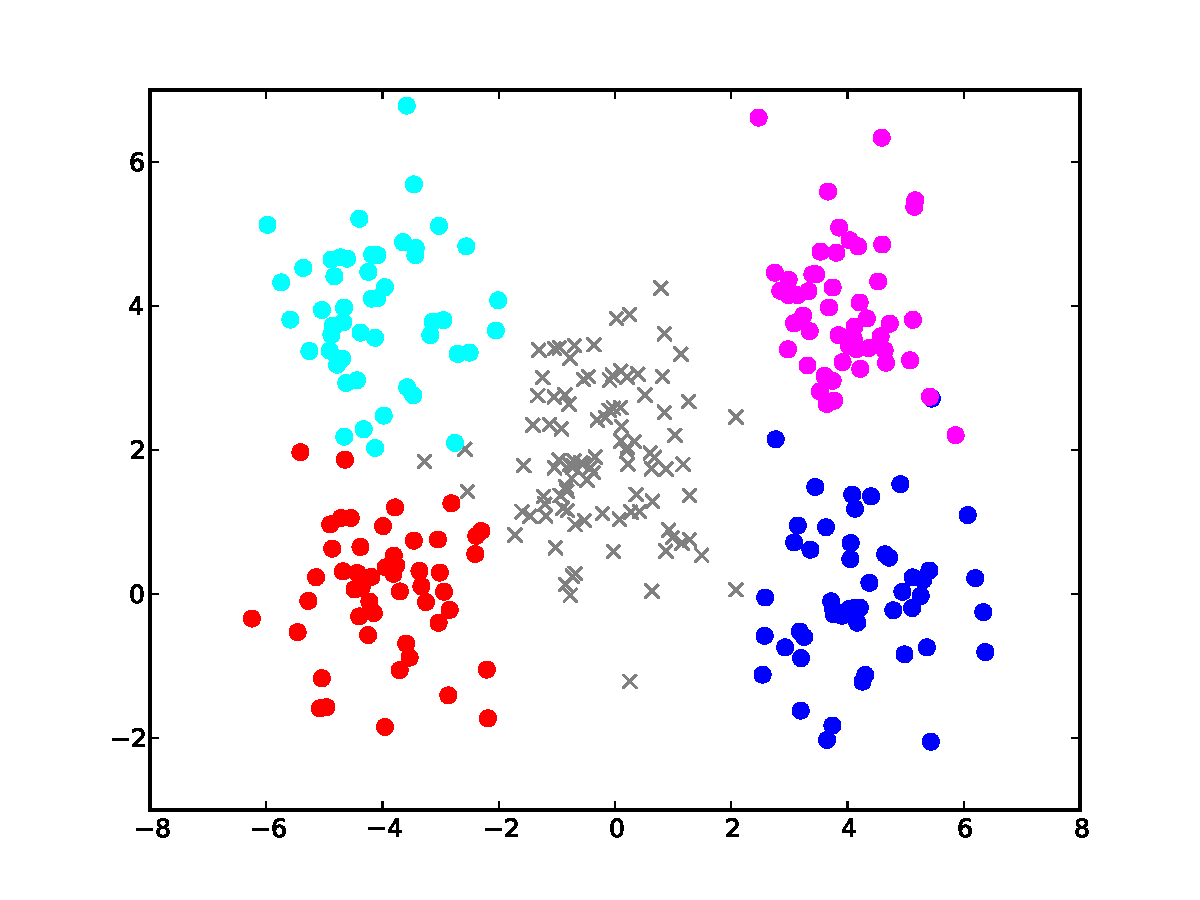
\includegraphics[width=0.92\textwidth]{before}}
\transdissolve<2>
\only<2>{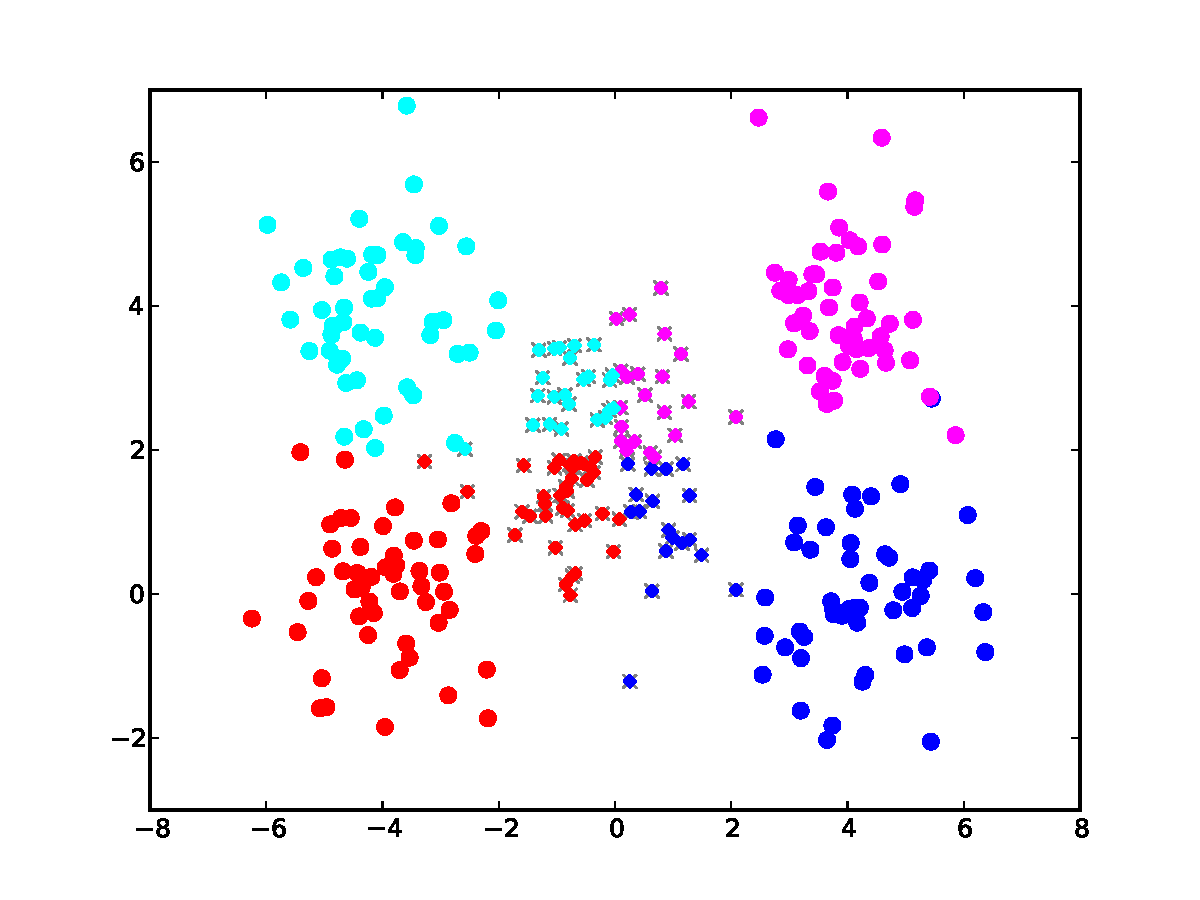
\includegraphics[width=0.92\textwidth]{after}}
\end{frame}

\begin{frame}{Пример классификации изображений}{CBCL (Center For Biological and Computation Learning, MIT) Face Database \#1}
\setlength\fboxsep{0pt}
\setlength\fboxrule{0.9pt}
\begin{itemize}
\item Классификация изображений 19x19 на два класса
\item Обучающая выборка (сокращённая):
$$
\overbrace {
\text{\fbox{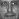
\includegraphics[width=0.7cm]{faces/face00001.png}}}
~
\text{\fbox{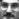
\includegraphics[width=0.7cm]{faces/face00002.png}}}
~
\text{\fbox{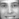
\includegraphics[width=0.7cm]{faces/face00003.png}}}
~
\text{\fbox{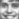
\includegraphics[width=0.7cm]{faces/face00004.png}}}
~
\text{\fbox{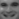
\includegraphics[width=0.7cm]{faces/face00005.png}}}
~
\text{\fbox{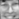
\includegraphics[width=0.7cm]{faces/face00006.png}}}
~
\text{\fbox{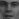
\includegraphics[width=0.7cm]{faces/face00007.png}}}
~
\text{\fbox{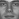
\includegraphics[width=0.7cm]{faces/face00008.png}}}
~
\text{\fbox{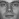
\includegraphics[width=0.7cm]{faces/face00009.png}}}
~
\text{\fbox{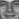
\includegraphics[width=0.7cm]{faces/face00010.png}}}
}^{{\color{green!40!black}\text{\bf всего 350 лиц}}}
$$
$$
\underbrace {
\text{\fbox{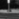
\includegraphics[width=0.7cm]{non-faces/B1_00001.png}}}
~
\text{\fbox{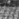
\includegraphics[width=0.7cm]{non-faces/B1_00002.png}}}
~
\text{\fbox{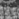
\includegraphics[width=0.7cm]{non-faces/B1_00003.png}}}
~
\text{\fbox{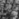
\includegraphics[width=0.7cm]{non-faces/B1_00004.png}}}
~
\text{\fbox{
\includegraphics[width=0.7cm]{non-faces/B1_00005.png}}}
~
\text{\fbox{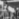
\includegraphics[width=0.7cm]{non-faces/B1_00006.png}}}
~
\text{\fbox{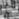
\includegraphics[width=0.7cm]{non-faces/B1_00007.png}}}
~
\text{\fbox{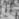
\includegraphics[width=0.7cm]{non-faces/B1_00008.png}}}
~
\text{\fbox{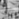
\includegraphics[width=0.7cm]{non-faces/B1_00009.png}}}
~
\text{\fbox{
\includegraphics[width=0.7cm]{non-faces/B1_00010.png}}}
}_{\color{red!40!black}\text{\bf всего 350 не лиц}}
$$

\item Тестовая выборка (сокращённая):
$$
\underbrace{
\text{\fbox{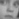
\includegraphics[width=0.7cm]{test/cmu_0000.png}}}
~
\text{\fbox{
\includegraphics[width=0.7cm]{test/cmu_0001.png}}}
~
\text{\fbox{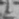
\includegraphics[width=0.7cm]{test/cmu_0002.png}}}
~
\text{\fbox{
\includegraphics[width=0.7cm]{test/cmu_0003.png}}}
~
\text{\fbox{
\includegraphics[width=0.7cm]{test/cmu_0004.png}}}
~
\text{\fbox{
\includegraphics[width=0.7cm]{test/cmu_0005.png}}}
~
\text{\fbox{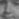
\includegraphics[width=0.7cm]{test/cmu_0006.png}}}
~
\text{\fbox{
\includegraphics[width=0.7cm]{test/cmu_0007.png}}}
~
\text{\fbox{
\includegraphics[width=0.7cm]{test/cmu_0008.png}}}
~
\text{\fbox{
\includegraphics[width=0.7cm]{test/cmu_0009.png}}}
}_{\text{\bf\color{main} всего 50 лиц и 50 не лиц}}
$$
\end{itemize}
\end{frame}

\begin{frame}{Классификация изображений: kNN}{CBCL (Center For Biological and Computation Learning, MIT) Face Database \#1}
%\begin{itemize}
%\item Простейший вариант: представление изображений как вещественных матриц и использование евклидовой нормы разности матриц как метрику
%\item Следующая зависимость точности от количества соседей $k$
~\\[-1.1cm]
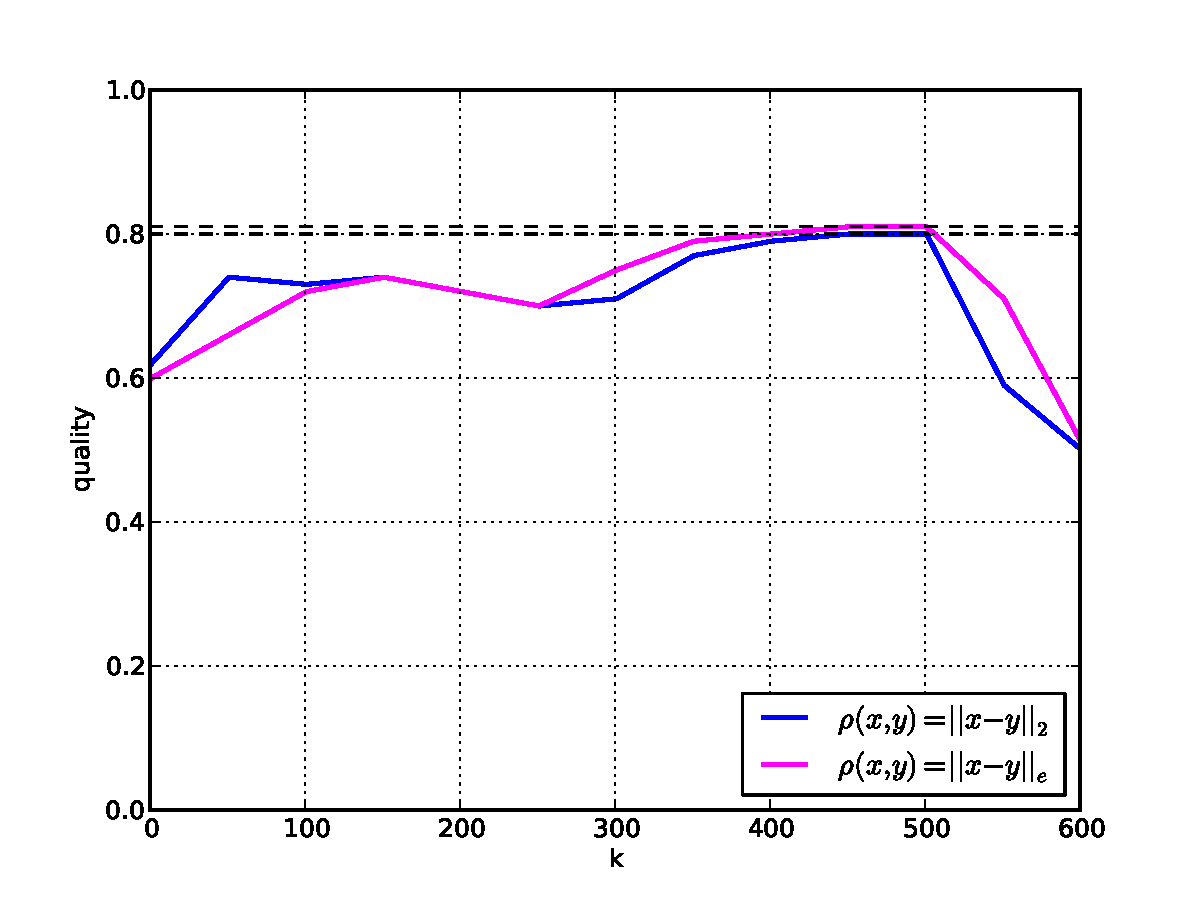
\includegraphics[width=\textwidth]{kNN-FNF}

%\end{itemize}
\end{frame}

\begin{frame}{Классификация изображений: парзеновские окна}{CBCL (Center For Biological and Computation Learning, MIT) Face Database \#1}
~\\[-1.1cm]
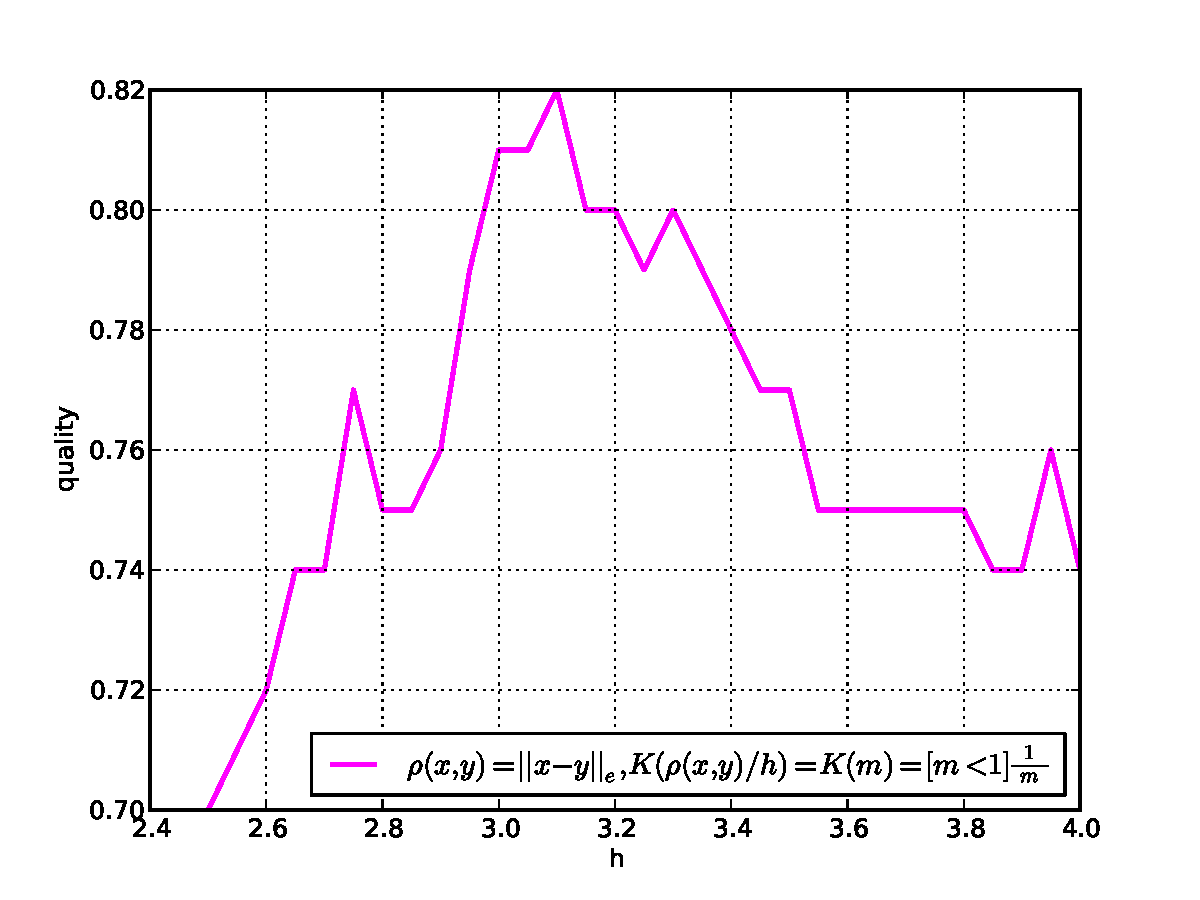
\includegraphics[width=\textwidth]{parzen}
\end{frame}

\begin{frame}{Способы повышения эффективности классификации}
\begin{itemize}
	\item Выбор более подходящей метрики
	\item Прореживание выборки (sampling)
	\item Фильтрация шумов
	\item Выбор эталонных объектов
	\item Понижение размерности данных
	\item Использование эффективных структур для хранения данных (kdTree, BallTree)

\end{itemize}
\end{frame}

%\begin{frame}{Эффективный поиск ближайшего соседа}{}
%\begin{itemize}
%\item {\bfc kd-деревья (k dimensional trees)} -- наиболее эффективная структура данных при поиске ближайшего соседа. Поиск по выборке, представленной в таком виде имеет асимптотику в среднем $O(\ln n)$.\\
%\begin{center}
%\definecolor{3rd1}{rgb}{0.2,0.8.0}
%\definecolor{3rd2}{rgb}{0,0.6,0.8}
%\definecolor{3rd3}{rgb}{0.6,0,0.8}
%\definecolor{3rd4}{rgb}{0.8,0.2,0}
%\definecolor{2rd1}{rgb}{0.2,0.9,0.8}
%\definecolor{2rd2}{rgb}{1,0.2,0.4}
%\begin{tikzpicture}
	\draw[dashed] (0,-2) -- (0,3); \draw (0,-2) node[color=black!40,opacity=1, ellipse, minimum height=0.2cm,minimum width=0.2cm,draw,fill,text=white] {A};
	\draw[dashed] (0,1.5) -- (-3,1.5); \draw (-2.5,1.5) node[color=2rd1,opacity=1, ellipse, minimum height=0.2cm,minimum width=0.2cm,draw,fill,text=white] {B};
	\draw (-0.7,2.2) node[color=3rd1,opacity=1, ellipse, minimum height=0.2cm,minimum width=0.2cm,draw,fill,text=white] {D};
	\draw (-1,-0.4) node[color=3rd2,opacity=1, ellipse, minimum height=0.2cm,minimum width=0.2cm,draw,fill,text=white] {E};
	\draw[dashed] (0,1) -- (3,1);
	\draw (2,1) node[color=2rd2,opacity=1, ellipse, minimum height=0.2cm,minimum width=0.2cm,draw,fill,text=white] {C};
	\draw (1,1.75) node[color=3rd3,opacity=1, ellipse, minimum height=0.2cm,minimum width=0.2cm,draw,fill,text=white] {F};
	\draw (1.75,-0.4) node[color=3rd4,opacity=1, ellipse, minimum height=0.2cm,minimum width=0.2cm,draw,fill,text=white] {G};
\end{tikzpicture}

%	\hfill
%\begin{tikzpicture}[anchor=north,rotate=-90,grow cyclic,shape=circle,very thick,level distance=16mm, cap=round]
	\tikzstyle{level 1}=[sibling angle=45]
	\tikzstyle{level 2}=[sibling angle=45]
	\tikzstyle{level 3}=[sibling angle=40]
	\tikzstyle{node}=[,fill,text=white]
	\tikzstyle{edge from parent}=[snake=expanding waves,segment length=0.8mm,
                              segment angle=7,draw]
\node [color=black!40] [node] {A} 
	child [color=2rd1] {
		node [node] {B}
			child [color=3rd1] {
				node [node] {D}}
			child [color=3rd2] {
				node [node] {E}}}
	child [color=2rd2] {
		node [node] {C}
			child [color=3rd3] {
				node [node] {F}}
			child [color=3rd4] {
				node [node] {G}}};
\end{tikzpicture}

%\end{center}
%\end{itemize}
%\end{frame}

%\begin{frame}{Нахождение оптимального значения параметра $k$ скользящим контролем}{}
%\begin{itemize}
%	\item Естественно, что алгоритм классификации должен правильно находить класс для каждого из элементов обучающей выборки
%	\item Минимизируя ошибку на обучающей выборке $T$ можно найти оптимальное $\tilde k$
%$$
%\tilde k = \arg \min_k \sum_{\left\{(x,f(x)\right\} \in T} [kNN(x,\!T\!,k) \ne f(x)],
%$$
%где $kNN(x,\!T\!,k)$ -- класс, определённый для точки $x$ в множестве $T$ с помощью построенного алгоритма, используя параметр $k$
%	\item В подавляющем большинстве случаев функционал будет иметь чёткий минимум
%\end{itemize}
%\end{frame}

\begin{frame}{Эффективность и вычислительная сложность}{}
	\begin{itemize}
	\item В целом, при адекватном выборе метрики и параметров методы ближайших соседей классифицируют объекты достаточно точно
	\item Вычислительная сложность алгоритма складывается из сортировки всей обучающей выборки $O(n \ln n)$ и обработки $k$ ближайших объектов за $O(k)$, однако большую часть времени занимает нахождение расстояний до объектов
	\item Классификация каждого нового объекта требовательна не только по времени, но и по памяти
	\item Как обработка, так и хранение объектов легко распределяется на несколько вычислительных узлов
	\end{itemize}
\end{frame}






%\begin{frame}{Ядро $K(\rho)$ и параметр $h$}
%\begin{itemize}
%	\item Ядра выбираются, как правило из стандартных: ядро Епанечникова, треугольное
%	\item Часто выбор ядра слабо влияет на качество классификации
%	\item Аналогично параметру $k$ в алгоритме $kNN$, минимизируя ошибку на %обучающей выборке $T$ можно найти  $\tilde h$
%$$
%\tilde h = \arg \min_h \sum_{\left\{(x,f(x)\right\} \in T} [\hat f_T(x,h) \ne %f(x)],
%$$
%где $\hat f_T (x,h)$ -- класс, определённый для точки $x$ в множестве $T$ с %помощью построенного алгоритма, используя ширину окна $h$
%	\item На практике можно выбирать простую функцию квадрата обратного %расстояния $K(\rho) = \frac{1}{\rho^2} [\rho<h]$, 
%\end{itemize}
%\end{frame}

%\begin{frame}{Пример классификации изображений с помощью парзеновского %классификатора}{CBCL (Center For Biological and Computation Learning, MIT) %Face Database \#1}
%
%\end{frame}

%\begin{frame}{Эффективность и сложность}{}
%\begin{itemize}
%	\item Сортировка обучающей выборки не нужна, это позволяет выполнять %классификацию существенно быстрее
%	\item Вся классификация производится за линейное по размеру выборки время %$O(n)$
%	\item Точность классификации существенно выше за счёт хорошей устойчивости %даже к множественным выбросам
%	\item По-прежнему, как и с kNN необходимо хранить всю выборку
%	\item Обработка хорошо параллелизуется и разделяется на подзадачи, что %делает алгоритм предпочтительным для высокопроизводительной классификации
%\end{itemize}
%\end{frame}

%\begin{frame}{Сравнение метрических алгоритмов}
%
%\begin{minipage}{0.45\textwidth}
%\begin{center}
%Обучающая выборка {\bf wines}\\[0.7cm]
%
%\begin{dataTable}
%{@{\hspace{1ex}} c @{\hspace{5ex}} c @{\hspace{1ex}}}%
%\color{white}{\bfМетод} & \color{white}{\bfТочность} \\ \midrule
%NN	&	0	 \\  \midrule
%kNN	&	0	 \\  \midrule
%wkNN	&	0 \\ \midrule
%kernel est.	&	0	 
%\end{dataTable}
%\end{center}
%\end{minipage}
%\hfill
%\begin{minipage}{0.45\textwidth}
%\begin{center}
%Обучающая выборка {\bf iris}\\[0.7cm]
%
%\begin{dataTable}
%{@{\hspace{1ex}} c @{\hspace{5ex}} c @{\hspace{1ex}}}%
%\color{white}{\bfМетод} & \color{white}{\bfТочность} \\ \midrule
%NN	&	0	 \\  \midrule
%kNN	&	0	 \\  \midrule
%wkNN	&	0 \\ \midrule
%kernel est.	&	0	 
%\end{dataTable}
%\end{center}
%\end{minipage}
%\end{frame}

\begin{frame}{What to know?}
\begin{itemize}
	\item Классификация: общий смысл и математическая формулировка задачи
	\item Принцип минимизации эмпирического риска (ERM), оптимальный с точки зрения ERM классификатор
	\item Аппроксимация апостериорной вероятности ближайшими соседями
	\item Методы ближайшего соседа, k ближайших соседей, k взвешенных ближайших соседей, парзеновских окон
	\item Пример классификации изображений ближайшими соседями
\end{itemize}
\end{frame}

\section{Support vector machines}
\subsection{}



\begin{frame}{Машины опорных векторов}{Support vector machines (SVM)}
\begin{itemize}
	\item Впервые представлен в начале 90-х, но основу метода составляют методы обобщённого портрета Вапника, разработанные ещё в 70-х
	\item Целое семейство методов решающее задачу классификации и регрессии
	\item Использует бинарный классификатор, разбивающий выборку на две части (и кое-что ещё)
	\item Многоклассовые классификаторы строятся как композиции бинарных
	\item Идея состоит в том, что положение гиперплоскости определяется положениями граничных точек -- опорных векторов
	\item Рассмотрим по мере усложнения: линейный SVM, регуляризованный SVM, ядровой SVM
\end{itemize}
\end{frame}

\begin{frame}{Линейный SVM}
\begin{itemize}
	\item Линейный алгоритм, классифицирующий некоторые объекты в евклидовом пространстве $\mathbb{R}^n = \mathcal{X}$ на классы $\mathcal{C}=\left\{ -1, +1 \right\}$, определяется следующим образом:
$$
f (x) =
\begin{cases} 
-1, & \langle w, x \rangle < w_0 \\
+1, & \langle w, x \rangle \geq w_0  
\end{cases}
$$
где $\langle \cdot , \cdot \rangle$ -- скалярное произведение.
	\item Задача обучения алгоритма сводится к нахождению вектора $w=\sum_i \alpha_i f(x_i) x_i$ и параметра $w_0$
	\item Такой классификатор хорошо подходит для линейно разделимых выборок (пересечения линейных оболочек объектов классов пустые)
\end{itemize}
\end{frame}


\begin{frame}{Линейный SVM: поиск параметров}
\begin{itemize}
	\item Из принципа структурной минимизации риска Вапником показано, что необходимо выбирать плоскость с наибольшим отступом (maximum margin):
	$$
	\frac{2}{\langle w,w \rangle} \to \max
	$$
	\item Нахождение такой плоскости -- решение задачи оптимизации
	$$
\frac{1}{2} \| w \|^2  \to \min
$$
при условии
$$
\forall i ~~ f(x_i) (\langle w, x_i\rangle + w_0 ) \geqslant 1
$$
	\item Линейная разделимость очень редко наблюдается на реальных данных
\end{itemize}
\end{frame}



\begin{frame}{Некорректность задачи в случае плохой разделимости: регуляризованной SVM}
\begin{itemize}
	\item Противоречие: разделить объекты надо -- разделить объекты невозможно
	\item Регуляризация задачи возможно позволит решить задачу с наименьшими <<потерями>>
	\item В 1995 году Вапник и Кортез предложили решать следующую задачу минимизации:
$$
\frac{1}{2} \| w \|^2 + C \sum_i \xi_i \to \min,
$$
где $\xi_i$ -- отступ объекта $x_i$ от границы
\end{itemize}
\end{frame}

\begin{frame}{Задача оптимизации: поиск положения разделяющей гиперплоскости}
\begin{itemize}
\item Минимизация регуляризованного функционала
$$
\frac{1}{2} \| w \|^2 + C \sum_i \xi_i \to \min
$$
при условии
$$
\forall i ~~ f(x_i) (\langle w, x_i\rangle + w_0 ) \geq 1 - \xi_i,\quad \xi_i \geq 0
$$
	\item Положение гиперплоскости определяется только объектами на границе -- опорными векторами (для них $\alpha_i \ne 0$)
	$$
	w = \sum_i \alpha_i f(x_i) x_i
	$$
	$$
	w_0 = - \frac{\max_{i, f(x_i) = -1} \langle w,x_i \rangle + \min_{i, f(x_i) = 1} \langle w,x_i \rangle}{2}
	$$
\end{itemize}
\end{frame}

\begin{frame}{}
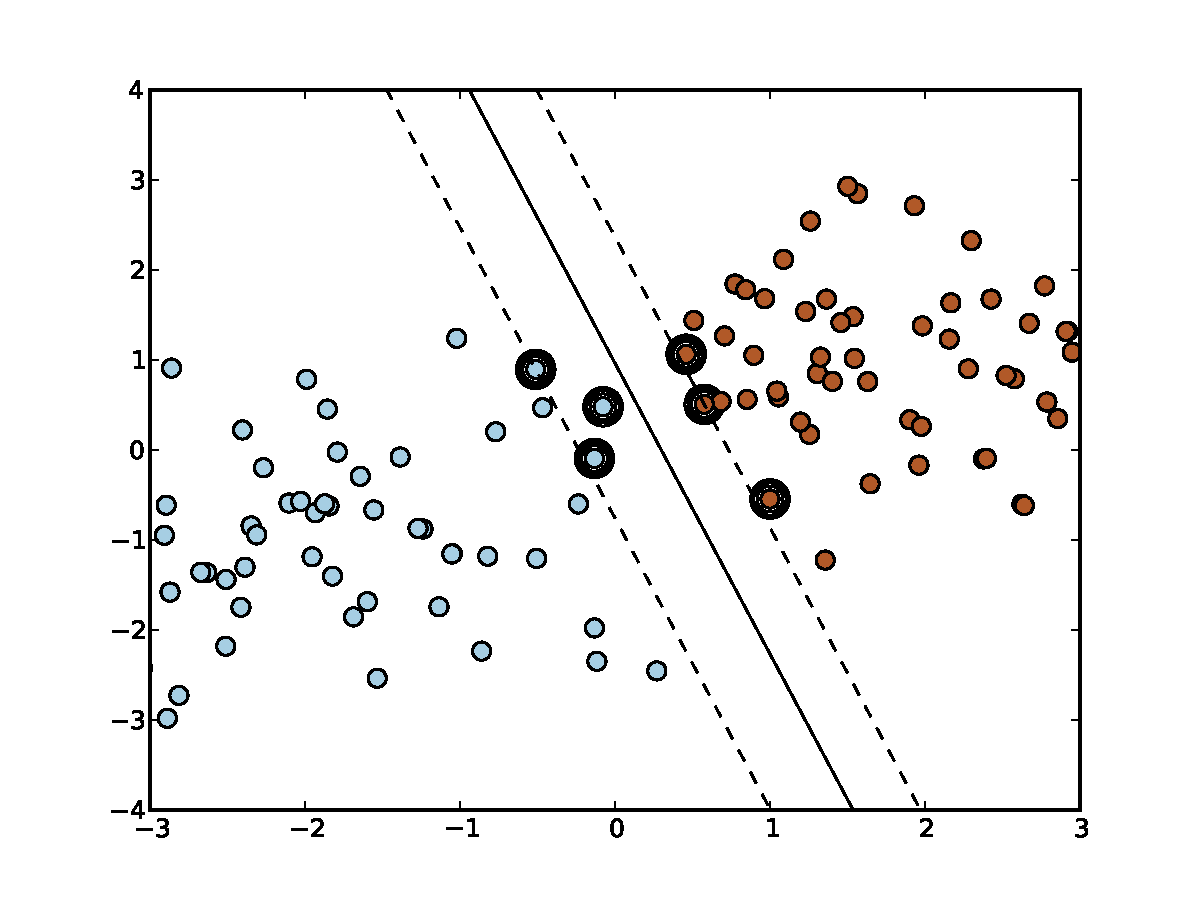
\includegraphics[width=\textwidth]{SVM-separable}
\end{frame}

%\begin{frame}{Машины {\bf опорных} векторов?}
%~\\[-0.7cm]
%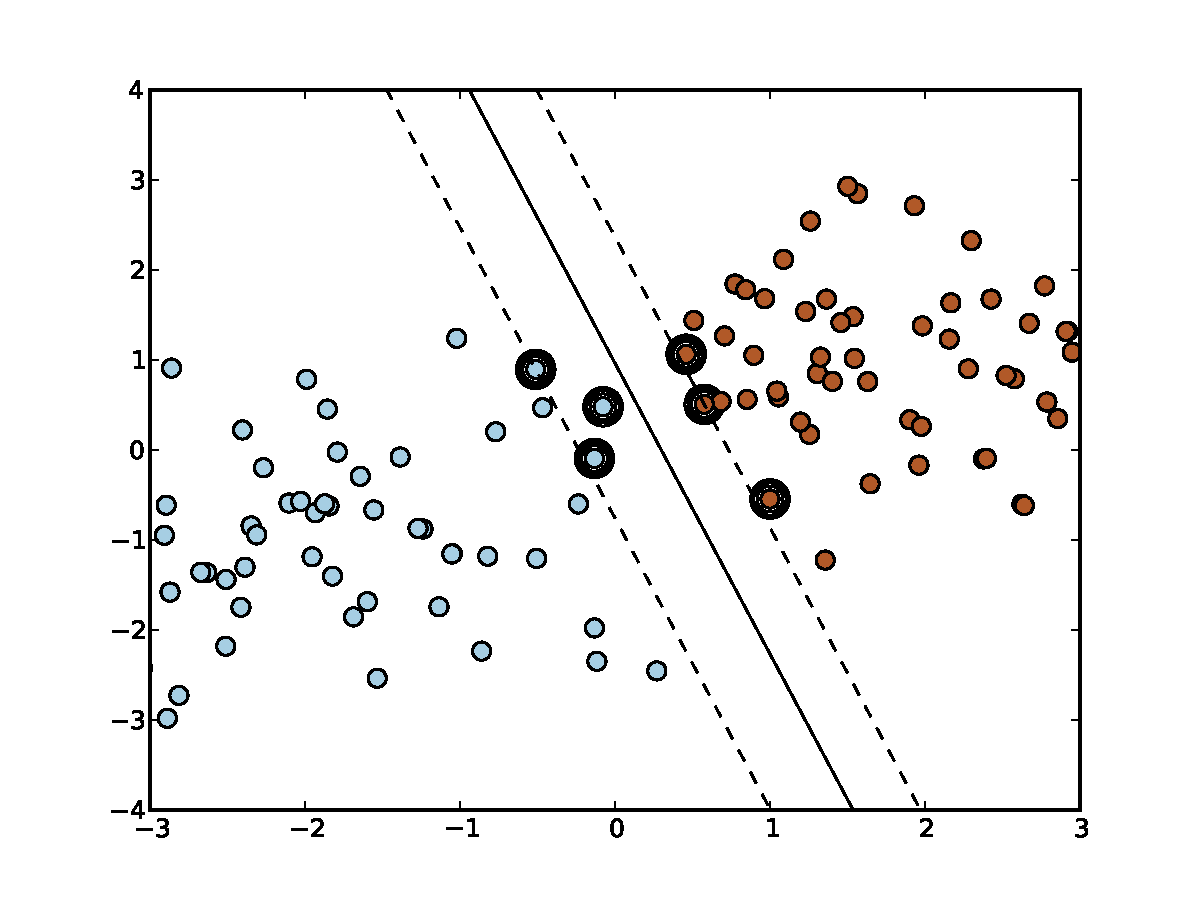
\includegraphics[width=\textwidth]{SVM-separable}
%
%\end{frame}

\begin{frame}{Sequential Minimal Optimization (SMO)}
\begin{itemize}
	\item Джон Платт из Microsoft Research в 1998 году разработал эффективный алгоритм поиска минимума функционала Лагранжа
	\item Задача квадратичного программирования разбивается на меньшие, решение которых ищется аналитически
	\item Алгоритм является итеративным и выполняет последовательные приближения по компонентами $\alpha_i$
	\item В результате скорость обучения классификации возрастает вплоть до тысячи раз (sic!)
\end{itemize}
\end{frame}

\begin{frame}{Некорректность задачи в случае неразделимости: спрямление пространства}
\begin{itemize}
	\item Разделяющая гиперплоскость для многих выборок совершенно бесполезна, даже регуляризация не позволяет найти <<хорошую>> гиперплоскость
	\item Любое пространство можно преобразовать в такое, в котором вся выборка линейно разделима -- проблема лишь в том, как его найти
	\item Отображение $\psi: \mathcal{X} \to \mathcal{H}$, повышающее размерность пространства объектов, может разделить выборку
	\item Вместо преобразования пространство достаточно изменить скалярное произведение (kernel trick): $$\langle x,y \rangle = K(x,y) = \psi(x)\psi(y)$$
	\item С помощью такого преобразования можно работать даже в бесконечномерных пространствах
\end{itemize}
\end{frame}

\begin{frame}{Выбор ядра спрямления}{}
\begin{itemize}
	\item Ядро -- функция, удовлетворяющее теореме Мерсера
	\item Примеры ядер:
	\begin{enumerate}
		\item Полиномиальное ядро $K_{\upalpha,c,d} (x,y) = (\upalpha x\cdot y + c)^d$\\
		\item Гауссовское (RBF) ядро $K_\beta (x,y) = \exp (-\beta \left\| x-y \right\|^2)$\\
		\item Сигмоидное ядро $K_{\upalpha,c}(x,y) = \th (\upalpha x \cdot y + c)$\\
		\item Ядро Коши $K_{\sigma} (x,y) = \dfrac{1}{1+ \frac{\| x-y \|^2}{\sigma}}$\\
		\item $K(x,y) = \sum_i \min (x_i, y_i)$
	\end{enumerate}
	\item Универсальных строгих правил для выбора ядра не существует
	\item Для подавляющего числа задач предпочтительнее RBF, но в некоторых случаях полиномиальное ядро лучше
	\item Ядро может быть построено с помощью композиции нескольких ядер:
	\begin{itemize}
	\item Неотрицательная линейная комбинация ядер -- тоже ядро
	\item Произведение ядер также ядро
	\end{itemize}
\end{itemize}
\end{frame}

\begin{frame}{Нелинейный SVM: выборка XOR}{С=10000, RBF kernel, $\nu=0.35$}
~\\[-1cm]
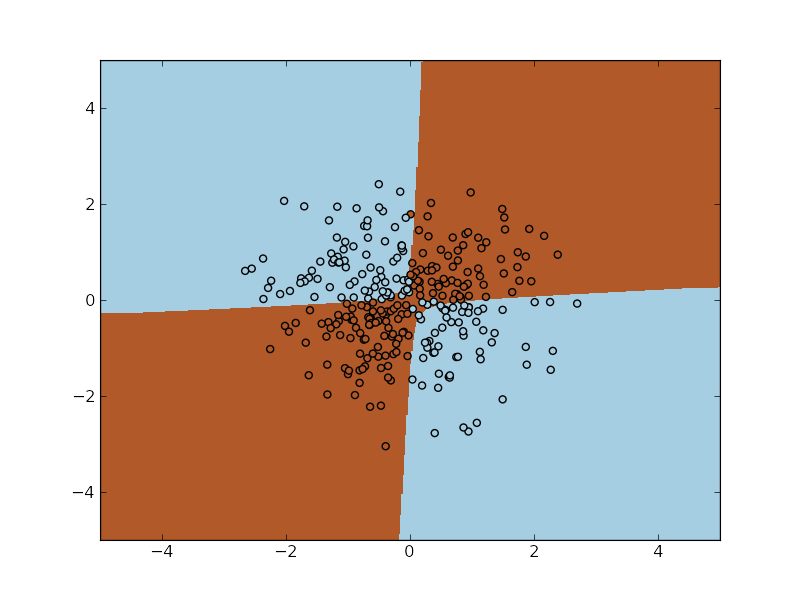
\includegraphics[width=\textwidth]{SVM-nonlinear.png}
\end{frame}

\begin{frame}{Многоклассовая классификация с помощью SVM}{}
\begin{itemize}
	\item Ранее рассматривалась только бинарная классификация, $\mathcal{C} = \left\{ -1 , +1 \right\}$, однако в реальном анализе данных гораздо чаще встречается многоклассовая классификация
	\item OVA (one versus all, один против всех) -- строится столько же классификаторов, сколько классов, каждый из которых противопоставляет бинарно один класс всем остальным
	\item При классификации объекта выбирается тот классификатор, в котором объект классифицируется <<увереннее>>, с максимальным отступом от гиперплоскости
\end{itemize}
\end{frame}

%\begin{frame}{Использование библиотеки libsvm в python}

%\end{frame}

%\begin{frame}{Сеточный поиск наилучших параметров}{Grid-search}

%\end{frame}

\begin{frame}{Эффективность алгоритма}
\begin{itemize}
	\item Построенный алгоритм не требует никаких вычислений, связанных с объектами обучающей выборки 
	\item Классификация выполняется достаточно быстро
	\item Само построение алгоритма классификации выполняется за существенное время и сильно зависит от реализации 
	\item SVM -- один из самых точных классификаторов
	\item На практике желательна нормировка входных данных
	\item Поиск наилучших значений параметров производится с помощью кросс-валидации или других процедур
\end{itemize}
\end{frame}

%\begin{frame}{Пример классификации изображений с помощью парзеновского классификатора}{CBCL (Center For Biological and Computation Learning, MIT) Face Database \#1}


%\end{frame}

\begin{frame}{What to know?}
\begin{itemize}
	\item Линейный SVM
	\item Регуляризация SVM при плохой линейной разделимости
	\item Kernel trick
	\item Sequential Minimal Optimization
	\item Мультиклассовая классификация с помощью SVM
\end{itemize}
\end{frame}


\section{}
\begin{frame}{Источники}
\begin{enumerate}
	\item Hastie T. et al, "The Elements of Statistical Learning: Data Mining, Inference and Prediction"
	\item Tom Mitchell "Machine learning"
	\item Золотых Н.Ю., <<Машинное обучение>>
	\item Воронцов К.В., <<Метрические алгоритмы классификации>>
	\item Воронцов К.В., <<Линейные алгоритмы классификации>>
	\item Burges C., "A Tutorial on Support Vector Machines for Pattern Recognition"
	\item Moore A., "Support Vector Machines"
	\item Hsu C.-W. et al, "A Practical Guide to Support Vector Classification"
	\item Platt J. "Sequential Minimal Optimization: A Fast Algorithm for Training Support Vector Machines"
	\item Cristianini N. "Support Vector and Kernel Machines"
\end{enumerate}
\end{frame}


\end{document}